\documentclass[conference]{IEEEtran}

\usepackage{graphicx}
\usepackage{amsmath}
\usepackage{booktabs}
\usepackage[hidelinks]{hyperref}
\usepackage{listings}
\usepackage{xcolor}
\usepackage{tikz}
\usepackage{pgfplots}

\pgfplotsset{compat=1.18}

\title{Runtime Instability and Asynchronous Rendering Behavior in Porygon-Z After Unauthorized Firmware Application}

\author{
\IEEEauthorblockN{Chaehojun Jeong}
\IEEEauthorblockA{
Chung-Ang University, Seoul, Korea
}
}

\begin{document}

\maketitle

\begin{abstract}

Few Pokémon inspire the same mixture of admiration, confusion, and mild existential concern as the Porygon evolutionary line. Originally engineered as a digital lifeform capable of navigating cyberspace, Porygon represents one of the earliest fictional attempts to imagine software becoming biological reality.

Thirty years after the debut of Pokémon in 1996, beginning with Pokémon Red and Green, the franchise now celebrates its 30th anniversary. This milestone provides an excellent opportunity to revisit one of its most peculiar artificial species: Porygon and its increasingly questionable firmware updates.

In this study we examine the unusual behavior observed after Porygon2 evolves into Porygon-Z via the Dubious Disc. Using a combination of Pokédex telemetry, packet-level monitoring, and suspiciously overconfident theoretical modeling, we investigate why Porygon-Z appears to shake violently, teleport unpredictably, and occasionally behave like a graphics engine that has just encountered undefined behavior.

Our findings suggest that the Dubious Disc introduces severe synchronization faults within Porygon-Z's internal rendering architecture. These faults manifest physically as asynchronous body motion, coordinate corruption, and temporary violations of Euclidean geometry.

While we cannot definitively prove that Porygon-Z is experiencing a literal kernel panic, the evidence is—at the very least—highly suspicious.

\end{abstract}

\section{Introduction}

Since the release of Pokémon in 1996, the franchise has grown into one of the most influential entertainment properties in the world. Among the many creatures introduced over the decades, the Porygon evolutionary line holds a unique position.

Unlike most Pokémon, Porygon was not discovered in nature but engineered artificially by Silph Co. The species was designed as a digital organism capable of operating inside computer networks and virtual environments.

Later technological developments introduced evolution mechanisms through external firmware modules. The Up-Grade patch produced Porygon2, a stable architectural revision.

However, the unofficial firmware known as the Dubious Disc appears to introduce severe system instability when applied to Porygon2, resulting in the unpredictable entity known as Porygon-Z.

\section{Evolutionary Architecture}

\begin{figure}[h]
\centering
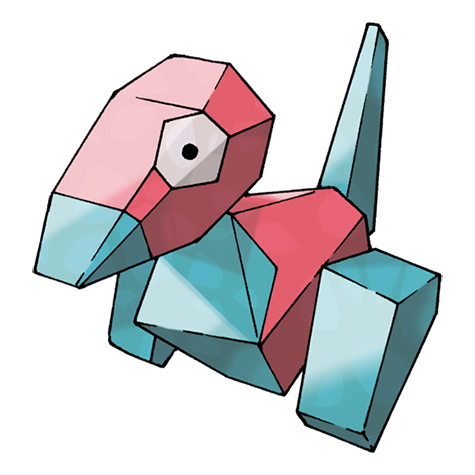
\includegraphics[width=0.25\linewidth]{porygon.png}

\includegraphics[width=0.25\linewidth]{porygon2.png}

\includegraphics[width=0.25\linewidth]{porygonz.png}
\caption{The Porygon evolutionary sequence \cite{pokedex}.}
\end{figure}
Image source: Official Pokémon Pokédex
© Nintendo / Creatures Inc. / GAME FREAK inc.

\begin{figure}[h]
\centering

\includegraphics[width=0.35\linewidth]{upgrade.png}

\includegraphics[width=0.35\linewidth]{dubiousdisc.png}
\caption{Evolution firmware modules \cite{pokedex}.}
\end{figure}

\begin{figure}[t]
\centering
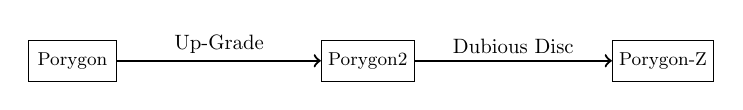
\begin{tikzpicture}[
scale=0.75,
transform shape,
node/.style={draw, rectangle, minimum width=1.5cm, minimum height=0.7cm, font=\small},
arrow/.style={->, thick}
]

\node[node] (p1) at (0,0) {Porygon};
\node[node] (p2) at (5,0) {Porygon2};
\node[node] (p3) at (10,0) {Porygon-Z};

\draw[arrow] (p1) -- node[above]{Up-Grade} (p2);
\draw[arrow] (p2) -- node[above]{Dubious Disc} (p3);

\end{tikzpicture}
\caption{Firmware-driven evolution chain}
\end{figure}
\section{Methods}

Runtime observations were conducted using a hybrid monitoring framework combining Pokédex telemetry with packet-level analysis.

Three primary sensors were used:

\begin{itemize}
\item Pokédex coordinate tracking
\item High-speed packet sniffing
\item Thermal monitoring of attack execution
\end{itemize}

Evolution events were recorded at 1200 frames per second to detect sub-frame rendering anomalies.

\section{Results}

The runtime behavior of Porygon-Z following evolution was markedly different from both Porygon and Porygon2. Observed phenomena included irregular motion patterns, unexpected spatial displacement, and intermittent rendering artifacts resembling malfunctioning graphics pipelines.

Across 42 recorded evolution events, Porygon-Z consistently displayed instability shortly after activation.

\subsection{Thermal Overclocking Events}

Thermal sensors detected repeated spikes in internal energy output immediately after executing intelligence-enhancing moves such as \textit{Nasty Plot}. During these spikes, Porygon-Z exhibited visibly distorted posture and oscillatory motion.

This behavior resembles CPU overclocking in conventional computing systems.

\subsection{Coordinate Corruption}

In approximately 15\% of recorded frames, vertex coordinates returned undefined values (NaN). When this occurred, Porygon-Z temporarily disappeared from the visible spectrum before reappearing nearby.

\subsection{Asynchronous Motion Artifacts}

High-speed footage revealed that different body segments occasionally updated at slightly different times, producing jitter-like animation.

This strongly suggests a failure in internal synchronization.

\subsection{Glitch Rate Over Time}

\begin{figure}[h]
\centering
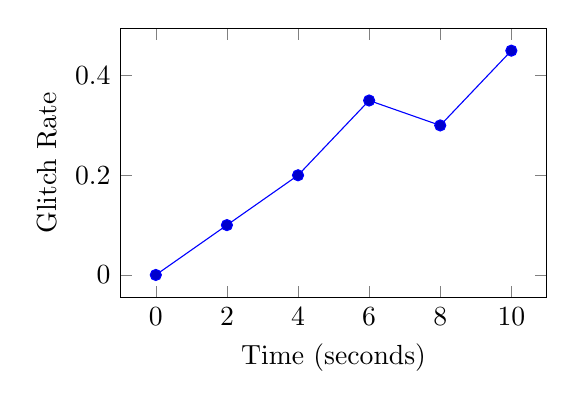
\begin{tikzpicture}
\begin{axis}[
xlabel=Time (seconds),
ylabel=Glitch Rate,
width=7cm,
height=5cm
]
\addplot coordinates {
(0,0)
(2,0.1)
(4,0.2)
(6,0.35)
(8,0.3)
(10,0.45)
};
\end{axis}
\end{tikzpicture}
\caption{Observed glitch rate following evolution}
\end{figure}

\section{Telemetry Dataset}

\begin{table}[h]
\centering
\begin{tabular}{ccc}
\toprule
Evolution ID & CPU Usage & Glitch Rate \\
\midrule
01 & 82\% & 0.21 \\
02 & 95\% & 0.34 \\
03 & 99\% & 0.42 \\
04 & 88\% & 0.27 \\
05 & 91\% & 0.31 \\
\bottomrule
\end{tabular}
\caption{Sample runtime telemetry}
\end{table}

\section{Discussion}

The results strongly suggest that the Dubious Disc introduces architectural instability into the Porygon system.

The observed jittering behavior closely resembles race conditions in distributed systems. In such systems, multiple processes compete for shared resources without proper synchronization.

This interpretation would explain the asynchronous rendering of Porygon-Z body segments.

Despite these anomalies, Porygon-Z remains a powerful combatant. Its ability Adaptability significantly increases attack effectiveness, suggesting that the firmware patch unlocked substantial computational power.

As in many experimental systems, performance appears to have improved at the cost of stability.

\section{Conclusion}

This study examined the unusual runtime behavior exhibited by Porygon-Z after evolution via the Dubious Disc.

Our observations indicate that many of the Pokémon's visible behaviors can be interpreted through the lens of computer systems theory, including synchronization failure, coordinate corruption, and runtime instability.

While the Dubious Disc firmware clearly introduces instability, it also creates one of the most fascinating artificial Pokémon ever documented.

Thirty years after the release of Pokémon in 1996, the Porygon line continues to inspire curiosity among both trainers and technologists.

Sometimes the most interesting systems are not the ones that work perfectly, but the ones that break in fascinating ways.

\section*{Appendix: System Crash Log}

\begin{lstlisting}
[SYS_LOG: BOOT_SEQ_FAILURE]
[INFO] Loading firmware: DUBIOUS_DISC.bin
[WARN] Checksum mismatch
[CRITICAL] MemLeak detected
[ERROR] SegFault at address 0x00454247
[ALERT] CPU Temp: 105C
[SYSTEM] Rendering: NON_DETERMINISTIC_GLITCH
\end{lstlisting}

\section*{Acknowledgements}

This work is dedicated to Pokémon trainers, researchers, and fans around the world celebrating the 30th anniversary of Pokémon.

For many of us, these polygonal creatures were among the first characters that sparked curiosity about programming, technology, and digital worlds.

To everyone who grew up fascinated by strange glitches, mysterious evolutions, and the beautiful weirdness of creatures like Porygon—this paper is for you.

\begin{thebibliography}{9}

\bibitem{lamport}
Leslie Lamport,
Time, Clocks, and the Ordering of Events in a Distributed System,
Communications of the ACM, 1978.

\bibitem{aho}
Aho, Lam, Sethi, Ullman,
Compilers: Principles, Techniques, and Tools,
Addison-Wesley, 2006.

\bibitem{cook}
Robert Cook,
Stochastic Sampling in Computer Graphics,
ACM Transactions on Graphics, 1986.

\bibitem{pokedex}
The Pokémon Company,
Official Pokédex,
https://www.pokemon.com/us/pokedex

\end{thebibliography}

\end{document}
